\speciestitle[(stored as an additional swath in the \texttt{L2GP-IWC}
  file).]{Cloud Ice Water Path}{IWP}{IWP}{%
  \item[Units:] g/m\cp2
  \item[Useful range:] MLS IWP is the ice water column above \mytexttilde6\,km
  \item[Contact: ] Alyn Lambert, \email{Alyn.Lambert@jpl.nasa.gov}}

\subsection{Introduction}

MLS standard IWP is retrieved from cloud-induced radiances (\Tcir) of the 240\nobreakdash-GHz window channel at 650\,hPa tangent pressure (see Figure~\ref{fig:IWPSketch}). It represents a partial column above \mytexttilde6\,km, and is stored in the \thisv L2GP IWC file as a separate swath. For the IWP retrieval, \Tcir\ is first converted to a near horizontal slant path (with a \mytexttilde3\degsym\ elevation angle) IWP ``hIWP'', using the modeled \Tcir--hIWP relation. The hIWP is then converted to the nadir IWP at the tangent point location, and interpolated to the MLS standard horizontal grid.

As noted in Section~\ref{sec:R2DutyCycling}, since May 2024 the \mbox{190\nobreakdash-GHz} radiometer is operated only intermittently. When that radiometer is turned off, in the absence of \ch{H2O} measurements, \emph{a priori} information for \ch{H2O} (based on climatological values) is used in the derivation of the IWP data product, adversely affecting the quality. Therefore, we do not recommend the use of IWP data during the periods that the \mbox{190\nobreakdash-GHz} radiometer is turned off. Further details are given in Section~\ref{sec:IWPScreening}.

\subsection{Resolution}

In the IWP ranges specified in the summary at the end of this section, each MLS measurement can be quantitatively interpreted as the average IWP for the volume sampled. The MLS IWP volume is a vertical column above \mytexttilde6\,km, with 60\,km and 7\,km along- and cross-track extent, respectively.

\subsection{Precision}

The precision values quoted in the IWP swaths do not represent the true precision of the data. The precision for a particular measurement must be evaluated on a daily basis using the method described in the screening section below. The 3\,g/m\cp2 precision given in the summary at the end of this section reflects \emph{typical values} for MLS IWP measurements.

\subsection{Accuracy}

The IWP accuracy is \mytexttilde50\%, as estimated from comparisons of the earlier \vii MLS data product with CloudSat and detailed analyses on the \vii error budget can be found in \citet{WuEtal:2009}.

\subsection{Data screening}
\label{sec:IWPScreening}
\begin{description}
  \item[Sensitivity:] The standard IWP product has a useful sensitivity up to 200\,g/m\cp{2} where MLS measurements can be quantitatively interpreted as the average IWP for the volume sampled.
  \item[Use Temperature Status, Quality and Convergence:] The user is recommended to screen the IWP data using the \texttt{Status} field in the collocated temperature profile to exclude bad retrievals \citep{SchwartzEtal:2008:Validation}. In other words, only IWP values for which Temperature \texttt{Status} is an even number should be used. Similarly, the users should only use IWP values where the corresponding Temperature profiles have \emph{Quality} of \CheckThis 0.9 or larger and \texttt{Convergence} less than \CheckThis 1.03.
  \item[Other screening:] the user is also recommended to screen the IWP data for significant cloud hits on a daily basis using the ``2$\sigma$, $3\sigma$'' method described in the IWC section (\ref{sec:StandardIWC}). The $3\sigma$ threshold is needed for cloud detection since a small percentage of clear-sky residual noise can result in a large percentage of false alarm in cloud detection.  Note that this screening step cannot provide an adequate correction for the lack of retrieved \ch{H2O} during the periods when the \mbox{190\nobreakdash-GHz} radiometer is turned off, and so the additional screening step on \ch{H2O} \texttt{Status} given below takes precedence.
  
          \item[Additional screening on \ch{H2O} \texttt{Status}:] As noted earlier, the quality of the IWP product is degraded when the \mbox{190\nobreakdash-GHz} radiometer is turned off, since only climatological \ch{H2O} is available in lieu of retrieved \ch{H2O}. In these circumstances, the IWP values cannot be quantitatively compared to measurements taken on surrounding days or in previous years when the \mbox{190\nobreakdash-GHz} radiometer was operational. Therefore, for quantitative studies, an additional screening step is recommended, whereby the \texttt{Status} field in the collocated \ch{H2O} profile is examined to remove affected IWP data. That is, only IWP values for which the \texttt{Status} flags of the corresponding \ch{H2O} profiles are an even number should be used in quantitative studies relying on IWP measurements.    
          
          \end{description}

\subsection{Artifacts}

High-latitude high-land surface can be mistakenly detected as a cloud when the atmosphere is very dry, allowing MLS 240\nobreakdash-GHz radiances to penetrate down to the surface. Surface emission/scattering can then reduce brightness temperature. Surface effects (e.g., over the highland over Antarctica) may introduce artificial IWP values as large as 10\,g/m\cp2. In addition, the geographical location of MLS IWP is currently registered at the tangent point, which is \mytexttilde2 profiles away from the actual location of the IWP column as shown in Figure~\ref{fig:IWPSketch}. The user needs to correct this offset by replacing the IWP location with the one at two profiles earlier.

\subsection{Comparisons with other datasets}
Compared to \vii IWP the \thisv IWP values are similar and the random noise is slightly smaller than in \vii (see Figure~\ref{fig:IWP}). Apart from the differences noted above, the MLS \thisv IWP is similar to the MLS \vii product described and validated in \citet{WuEtal:2009}. A revised validation paper for IWP is not planned in the near future and users are advised to read \citet{WuEtal:2009} for more information.

Comparisons between \vii MLS and CloudSat IWP showed good agreement with PDF differences $<$50\% for the IWP range specified in the summary at the end of this section.

\subsection{Desired improvements for future data version(s)}

The IWP retrieval in \thisv is a simple first-order conversion, applied independently to each \Tcir\ measurement. Future development work on the MLS IWP retrieval should consider implementing a 2-D cloudy-sky radiative transfer model. This will allow IWP to be retrieved jointly with the \Tcir\ measurements from adjacent scans.

\subsection{Summary for IWP}
\begin{description}
  \item[IWP column bottom:] \screeningrule{6\,km (estimated from MLS radiative transfer model calculations).} The calculation of the bottom height of the IWP column depends on the tropospheric water vapor loading and on the IWP itself and is discussed in \citet{WuEtal:2009}.
  \item[Typical precision:] \screeningrule{3\,g/m\cp2 is the typical 1$\sigma$ precision.} The precision for a particular measurement must be evaluated on a daily basis using the method described in the text.
  \item[Accuracy:] \screeningrule{50\% (estimated from comparisons with CloudSat)}
  \item[Resolution:] \screeningrule{60\,km along track, 7\,km across track (the volume of air sampled by MLS)}
  \item[Valid IWP range:] \screeningrule{$\le$200\,g/m\cp2} This is the range where the stated precision, accuracy and resolution are applied. In this range MLS measurements can be quantitatively interpreted as the average IWP for the volume sampled. IWP values above this range, currently giving qualitative information on cloud ice, require further validation for quantitative interpretation.
\end{description}

\begin{figure}
  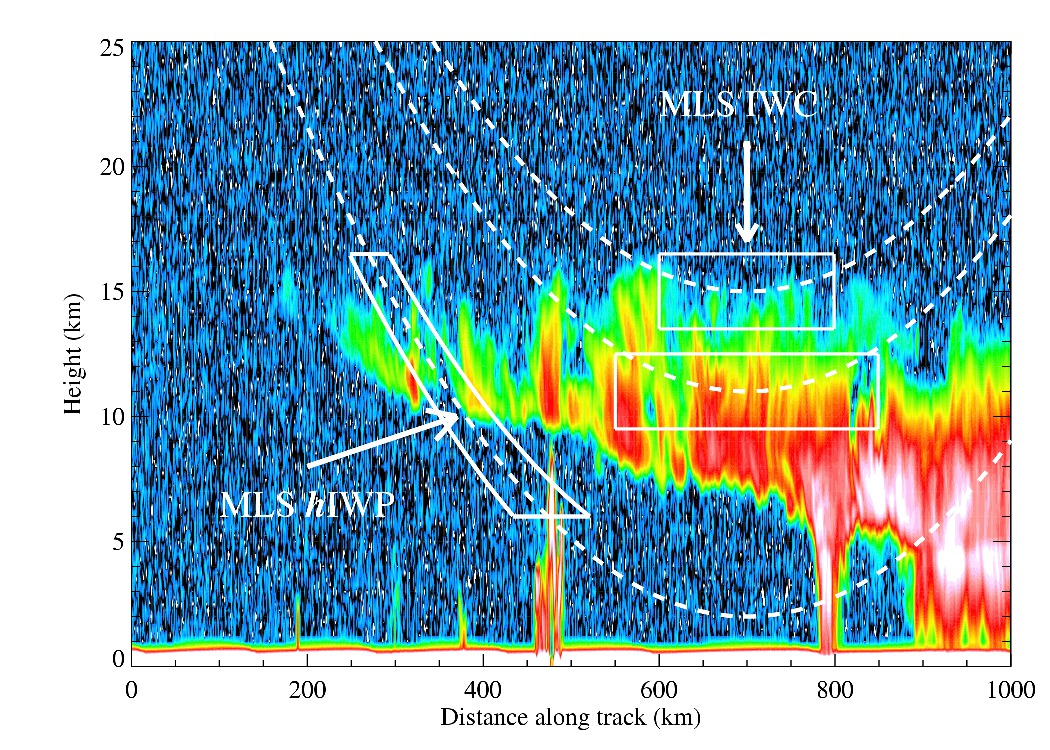
\includegraphics[width=\textwidth]{figures/iwp-figure-bitmap.jpg}
  \caption{Diagram to illustrate the MLS IWC and IWP measurement. The dashed lines are the MLS tangential beams. At high tangent heights, the beams penetrate through the limb and become sensitive to a volume-averaged IWC, whereas, at low tangent heights, the MLS beams cannot penetrate through the limb due to strong gaseous absorption and become only sensitive to a partial slant column of IWP, with a shallow (\mytexttilde3\degsym) angle, ``hIWP''.  Note that the actual volume of the air represented by hIWP is centered \mytexttilde300\,km away from the tangent point, or \mytexttilde2 profiles from the location of the nominal profile.}
  \label{fig:IWPSketch}
\end{figure}

\begin{figure}
  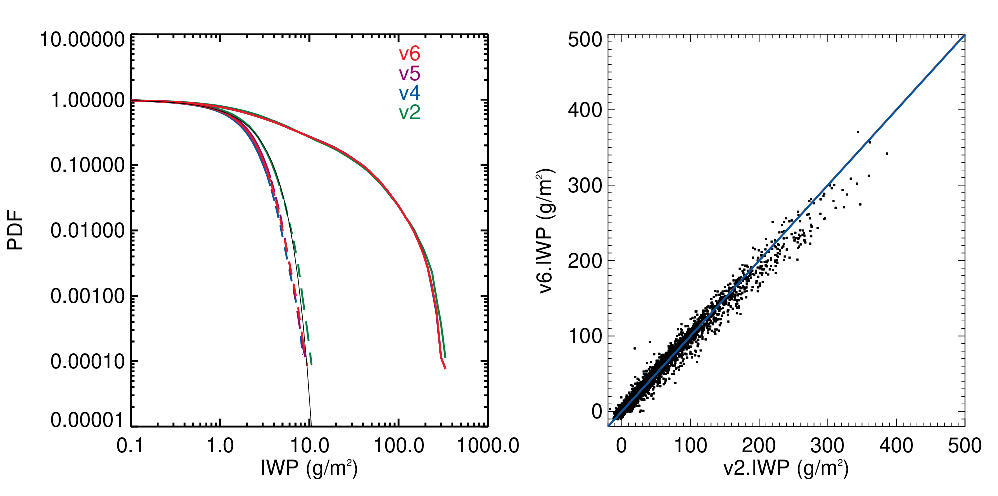
\includegraphics[width=\textwidth]{figures/IWP-240-v6-dataqual-JUN2009}
  \caption{MLS v6, v5, v4 and v2 IWP comparisons for June 2009.  (a) Left: Probability density functions (PDF) (v6 (red), v5 (purple), v4 (blue) and v2 (green)) with dashed lines showing the corresponding noise levels (obtained by folding the negative IWP values about the origin) and the thin black lines representing the gaussian error function. (b) Right: Scatter plot of IWP \thisv vs v2 (black points) with a linear fit to the data shown as a blue line and lying practically along the 1:1 line.}
  \label{fig:IWP}
\end{figure}
